\learn{7}{11.01}
\begin{notation}
    在模型下,对样本阳/阴性的预测结果为一个概率$p \in [0,1]$ ,通过设定一个阈值$m$ 来区分由模型预测的结果;在该阈值下,计算查全率和查准率,绘制一个点;设定不同的阈值,将所有点连接,得到$\bm{P}-\bm{R}$ 曲线
\end{notation}
\begin{figure}[htbp]
    \centering
    \caption{$\bm{P}-\bm{R}$ 曲线}
    \label{fig:P-R}
    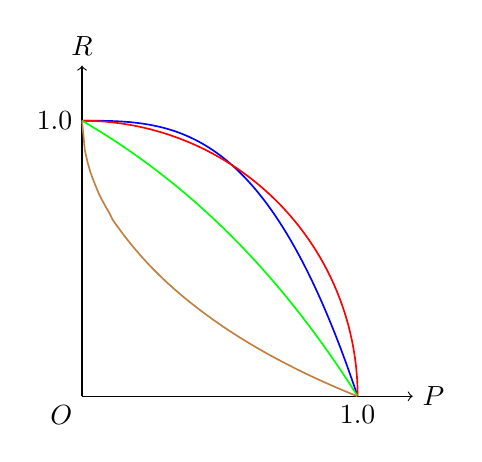
\begin{tikzpicture}[yscale=3.5,xscale=3.5]
        % Axis
        \draw [->] (0,0)--(1.2,0) node [right] {$\bm{P}$};
        \draw [->] (0,0)--(0,1.2) node [above] {$\bm{R}$};
        \node [anchor=north east] at(0,0) {$O$};

        \draw [color=blue,semithick,domain=0:1,samples=100] plot (\x, {1-\x^3});
        \draw [color=red,semithick,domain=0:1,samples=2000] plot (\x,{sqrt(1-\x^2)});
        \draw [color=green,semithick,domain=0:1,samples=100] plot (\x,{-(exp(\x)-1)/(e-1)+1});
        \draw [color=brown,semithick,domain=0:1,samples=100] plot (\x,{1-(ln(\x+sqrt(\x^2+1))/ln(1+sqrt(2)))^0.5});
        \node [below] (10) at(1,0) {$1.0$};
        \node [left] (10) at(0,1) {$1.0$};
    \end{tikzpicture}
\end{figure}


